\chapter{Experimental validation in real-world scenario}
\label{ch:real_world_application}
This chapter details the validation of the proposed methods in a real world scenario. Specifically, Section~\ref{sec:real_world_exp_setting} describes the experimental setup. Section~\ref{sec:real_world_dataset} discusses the dataset used to train the system. Finally, Section~\ref{sec:real_results} presents the results obtained.

\section{Experimental Setting}
\label{sec:real_world_exp_setting}
In this section, the experimental setup is explained and defined. Figure \ref{fig:workspace} illustrates the workspace where the robot operates, and compares it to the corresponding simulation environment. As can be observed, the simulation environment closely resembles the real-world counterpart. Both environments consist of the same robot agent, with identical camera configurations and workspace setup.

\begin{figure}[t]
    \centering
    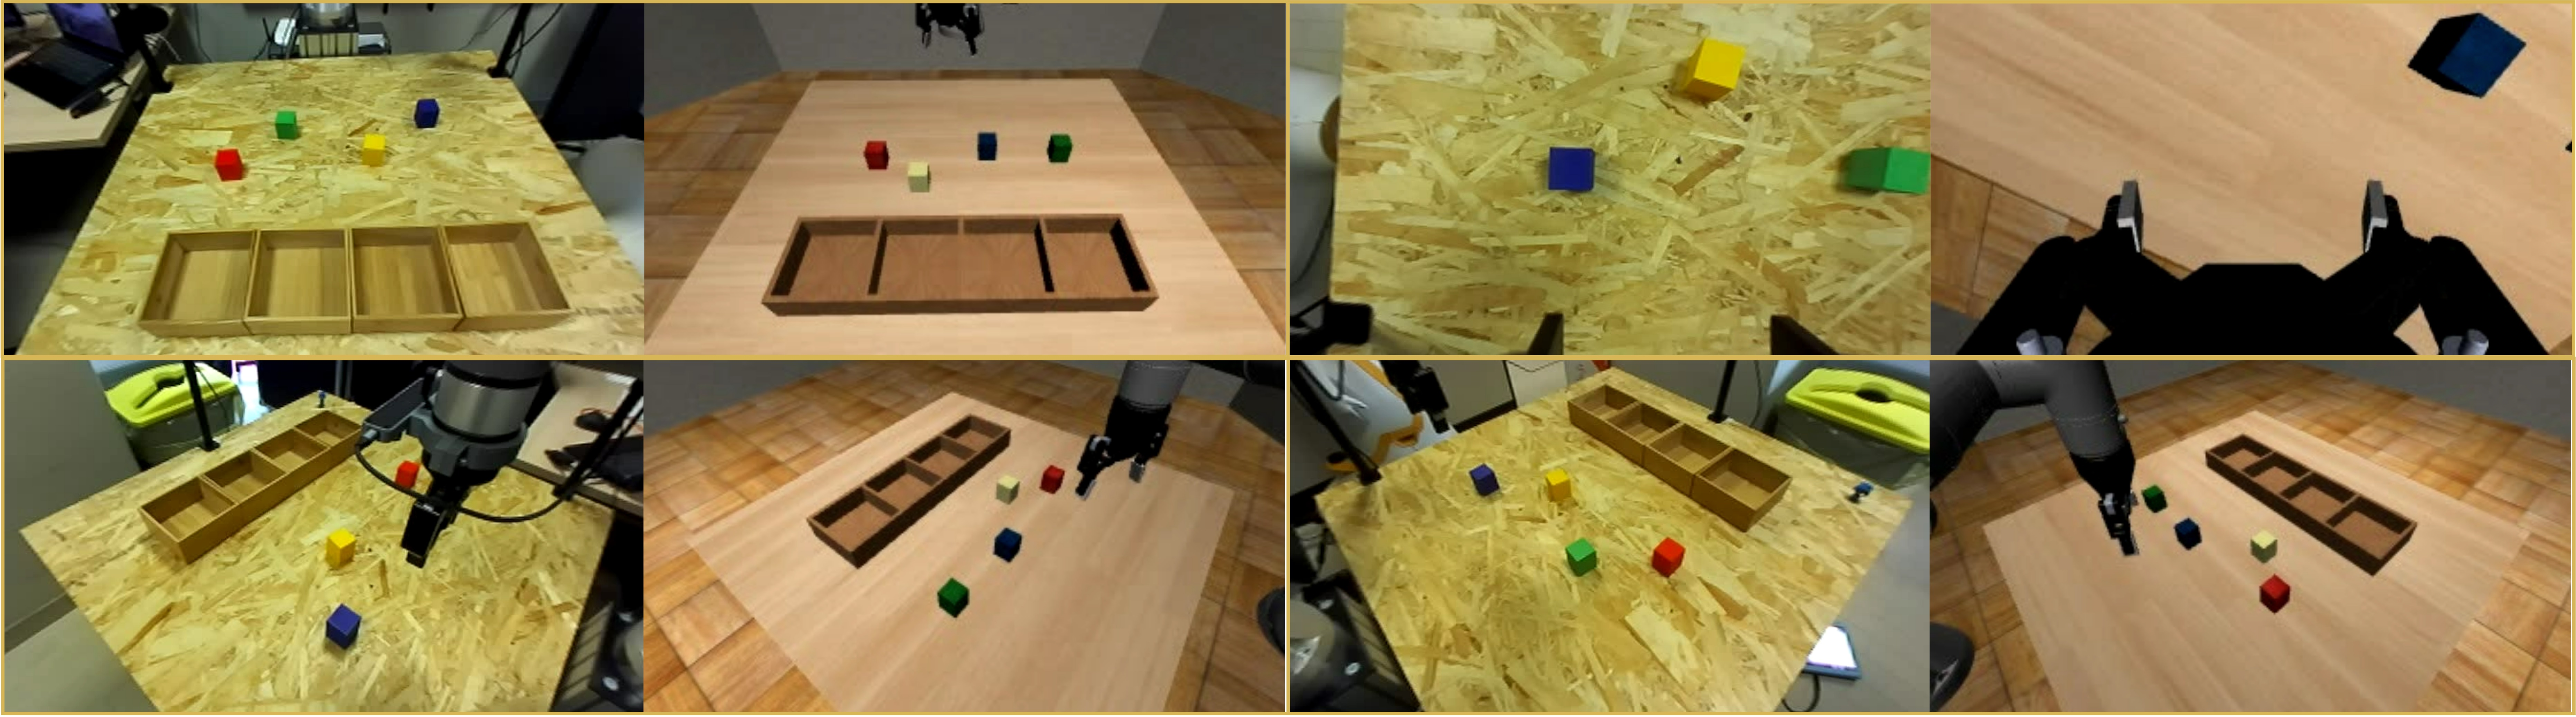
\includegraphics[width=1.0\textwidth]{figures/images/ch5/workspace.jpg}
    \caption{Workspace comparison between real-world (left) and simulated (right) scenarios. Images are taken from the frontal camera (Top-Left), the gripper camera (Top-Right), lateral-left camera (Bottom-Left) and lateral-right (Bottom-Right).}
    \label{fig:workspace}
\end{figure}

Specifically, the experimental setup includes:
\begin{itemize}
    \item The Universal Robots UR5e robot \cite{ur5e}, equipped with the Robotiq 2F-85 gripper \cite{robotiq}, which acts as the agent.
    \item Four Zed-Mini stereo cameras \cite{zed}, one camera is mounted on the gripper, while the remaining three are positioned around the robot to ensure complete coverage of the workspace.
    \item A 100$\times$100 cm working table.
\end{itemize}

The reason for maintaining a high similarity between the real-world and simulation environments is to evaluate the potential for pre-training the model on a large and comprehensive simulation dataset, followed by fine-tuning on a smaller and incomplete real-world dataset. This approach allows leveraging the advantages of simulation for initial training while adapting the model to real-world conditions with minimal additional data.

\section{Dataset}
\label{sec:real_world_dataset}
For the real-world validation, the focus will be on testing the model on the \textbf{multi-variation} \textit{Pick-Place} tasks, focusing on a smaller set of variations compared to the complete 16 variations described in Section \ref{sec:cod_dataset}.

\begin{figure}[t]
    \centering
    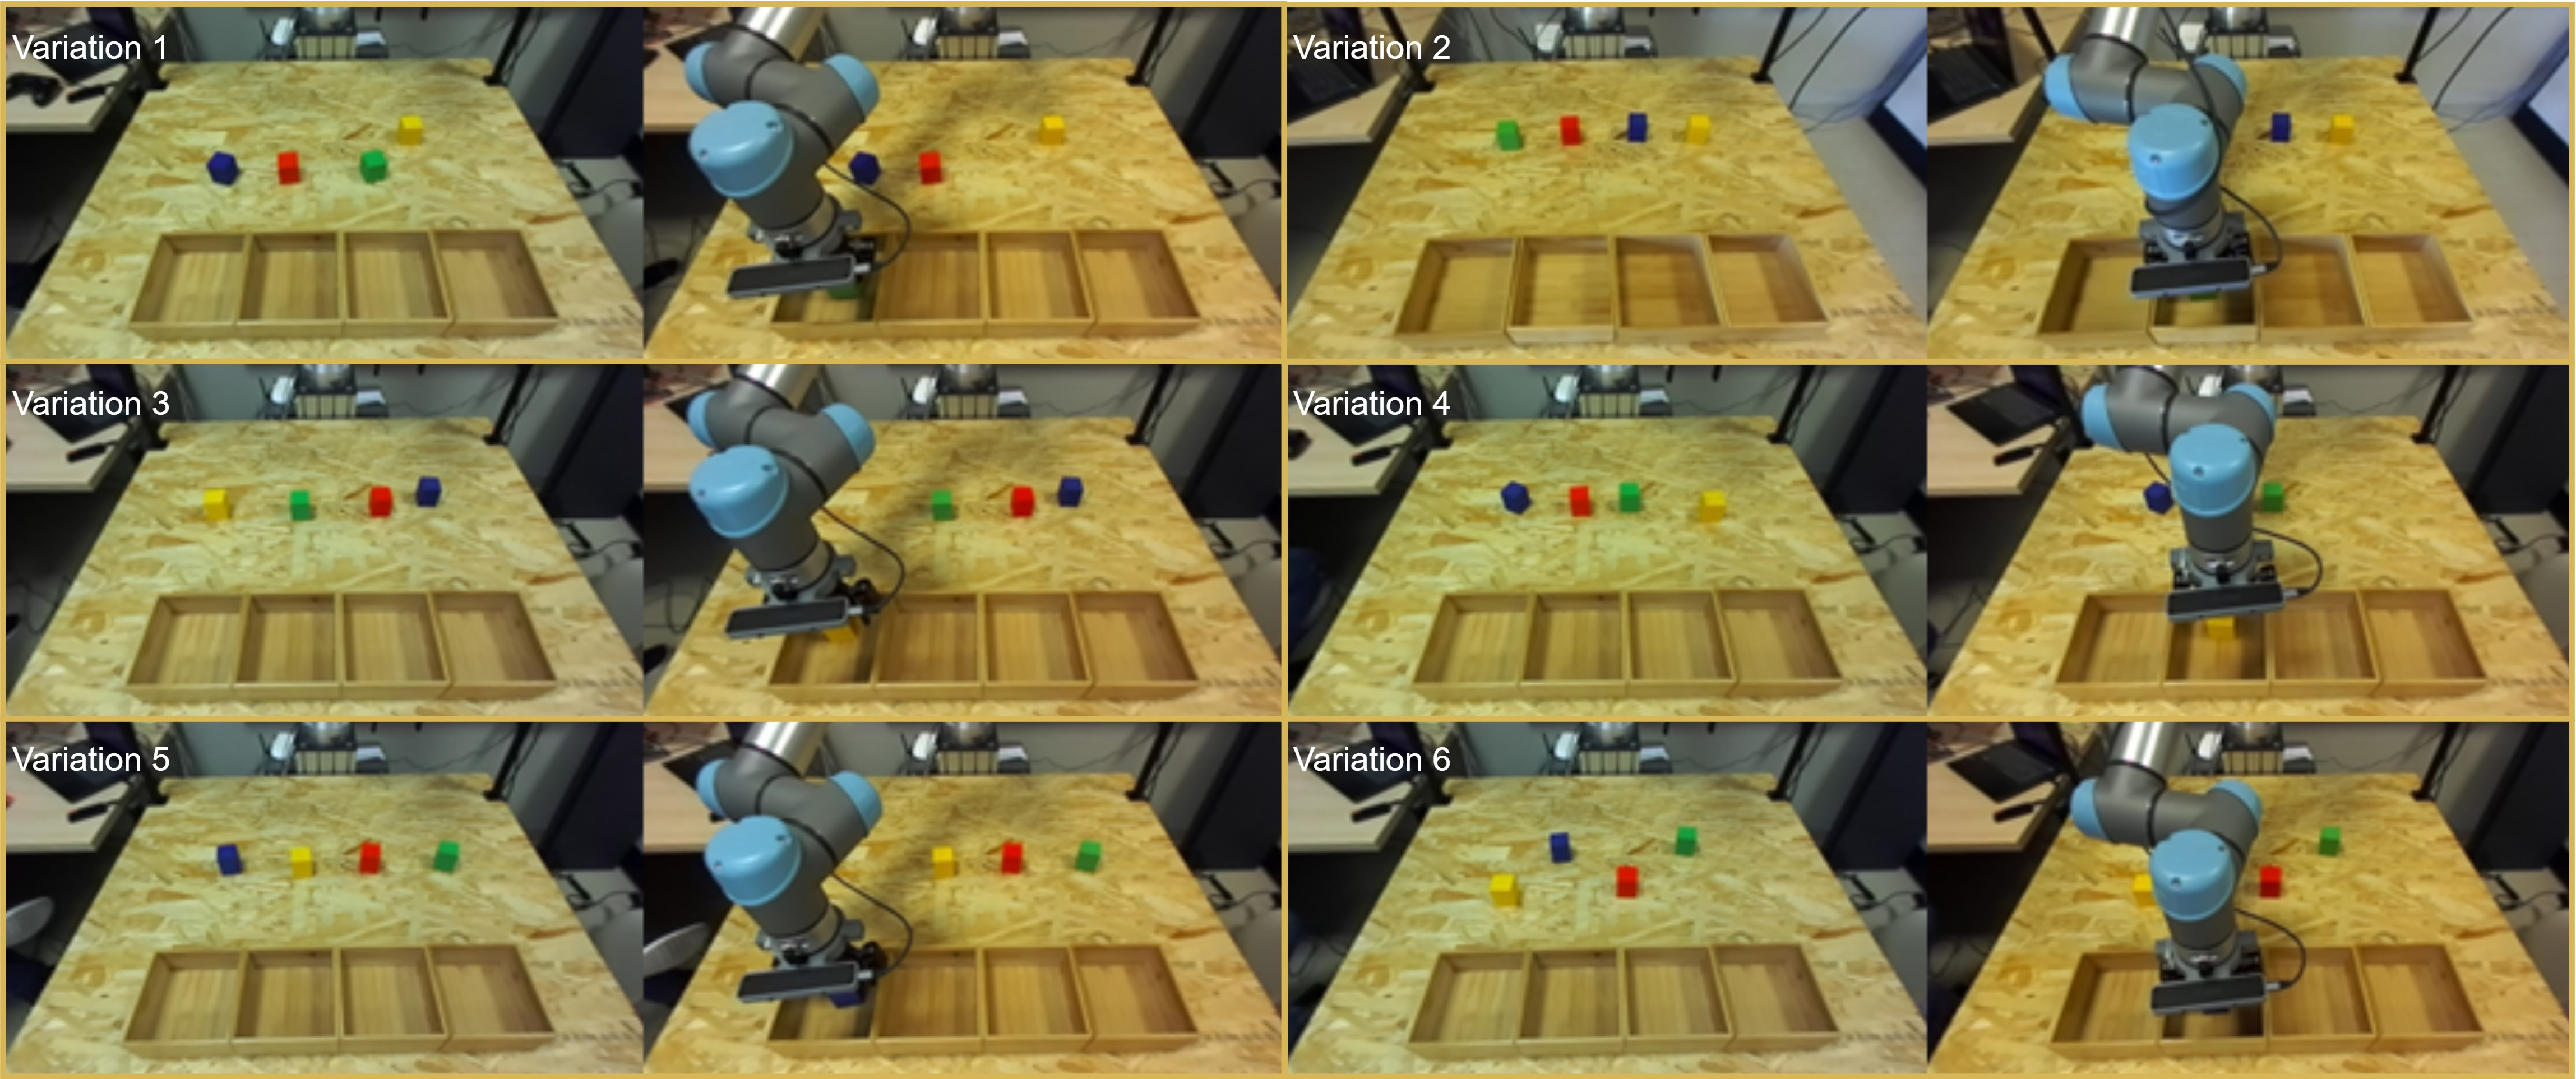
\includegraphics[width=1.0\textwidth]{figures/images/ch5/real_world_dataset.jpg}
    \caption{Set of variations used in the real-world robot evaluation. For each variation, the first and last frames are provided}
    \label{fig:real_world_dataset}
\end{figure}


Figure \ref{fig:real_world_dataset} represents the 6 variations used in the real-world validation. As can be noted, these are essentially the first six variations of the Pick-Place Task used in the simulation environment.

A preliminary dataset composed of \textbf{40 trajectories} for each variation has been collected by teleoperating the robot with a console controller. Regarding the object placement, the same algorithm described in Section \ref{sec:ocpl_dataset} was applied. This means that the set of 4 bins ($15 \times 15 \times 7$ cm) was fixed in position, while the 4 boxes ($4 \times 4 \times 6$ cm) could vary in their position within a region of $60$ cm in length and $15$ cm in height. 

In this extensive placement area, a specific protocol was implemented for collecting the trajectories. The protocol dictates how the objects are positioned within the picking region. The various placements of the target object are illustrated in Figure \ref{fig:box_placement}. Although the workspace may appear somewhat limited, this dataset is the first real-world dataset in the context of Visual-Conditioned Imitation Learning to encompass such a large operational space. In contrast, other works are either restricted to simulation environments \cite{dasari2021transformers_one_shot,mandi2022towards_more_generalizable_one_shot} or present very simple scenarios where objects are placed in a much smaller area \cite{mandlekar2022matters}.
\begin{figure}[t]
    \centering
    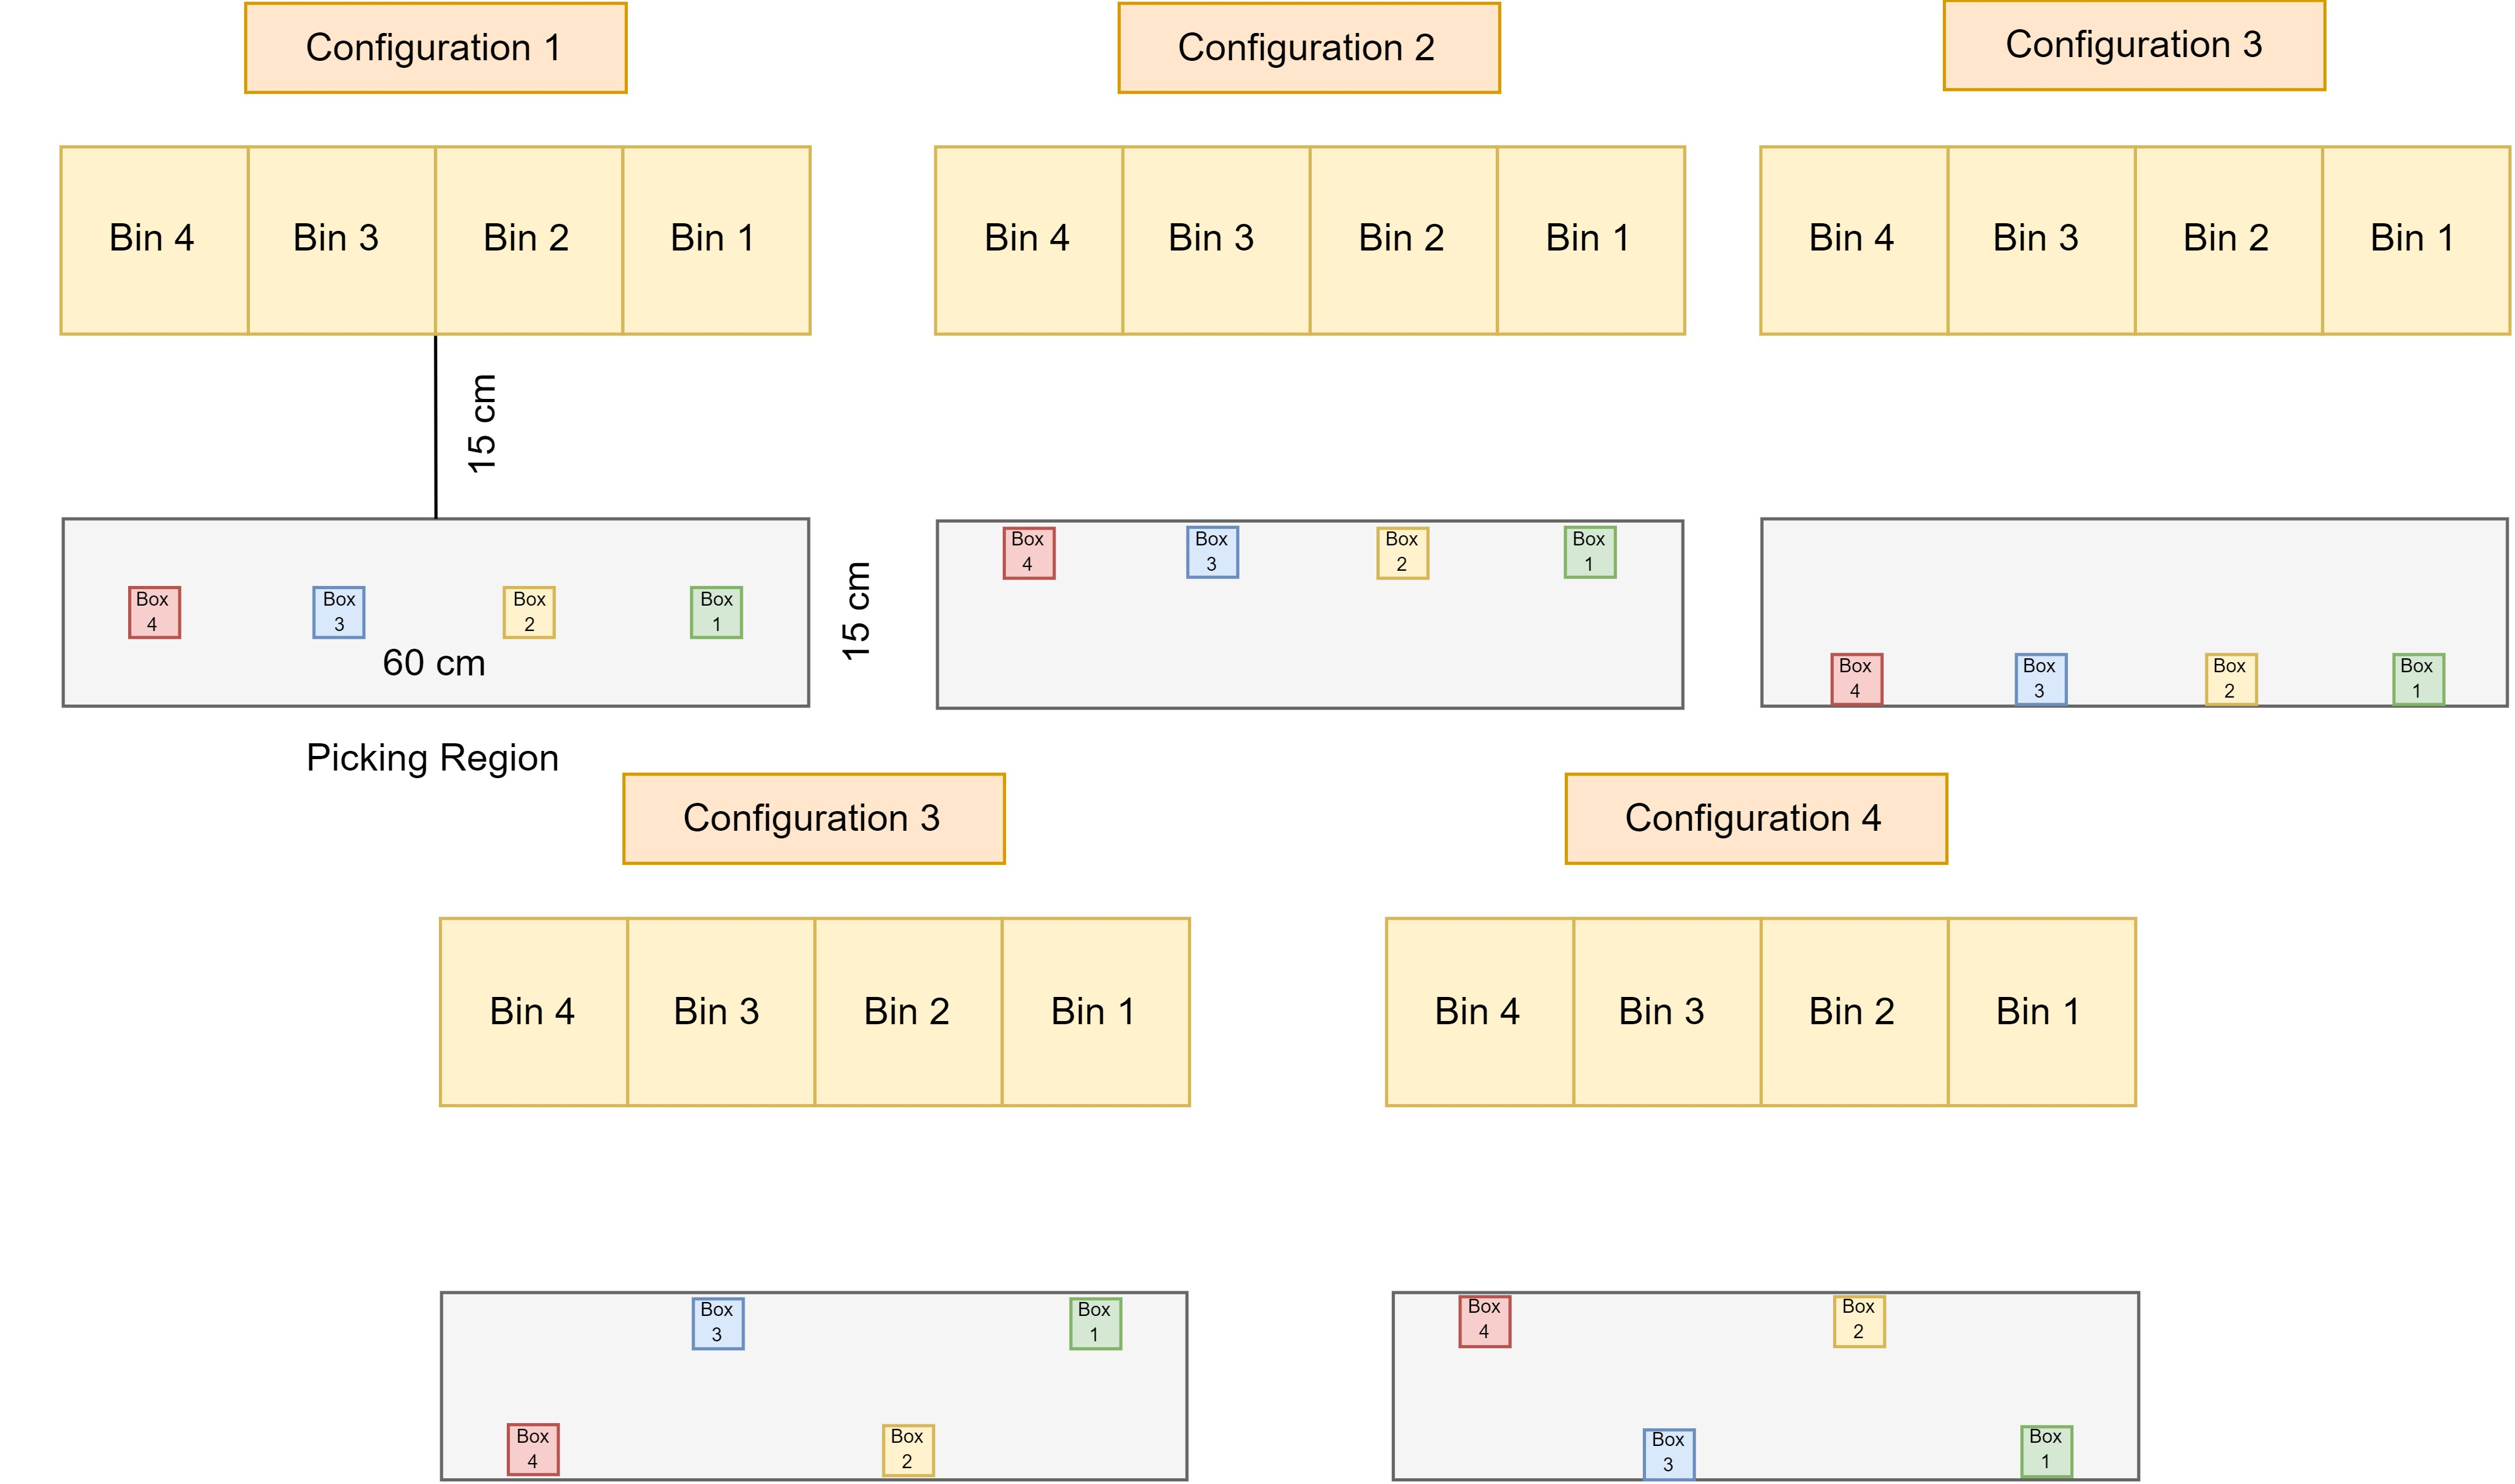
\includegraphics[width=0.8\textwidth]{figures/images/ch5/box_placement.jpg}
    \caption{Placement configuration used for the trajectory collection. For each placement configuration, 4 trajectories were collected. The target object initially starts at the rightmost position, and in each subsequent trajectory, the box is moved to the adjacent position. This process is then repeated twice, each time with a different object orientation, resulting in a total of 40 trajectories for a given configuration.}
    \label{fig:box_placement}
\end{figure}

% \smalltodo{add figure}
% \smalltodo{add figure}
Trajectories are collected through teleoperation the robot is controlled in its operational space, with the controller that sends continous velocity commands on a specific axis, this velocity command is defined by the value read by the controller's potentiometers.
During teleoperation different informatin are recorded:
\begin{itemize}
    \item \textit{Images} from the front, laterals and gripper cameras, both RGB and Depth images are recorded.
    \item \textit{Proprioceptive information} like joints positions and velocities.
    \item \textit{Trajectory state}, which is manually changed by the human operators based on the task state. The phases are:
        \begin{enumerate}
            \item \textit{Start}, this phase starts at the beginning of the trajectory till the robot gripper is perpendicular to the target object.
            \item \textit{Approaching}, this phase starts when the robot approaches the target object with its discending movement.
            \item \textit{Picking}, this phase is characterized by the gripper that is ready to be closed to pick the object, and contains the closing command.
            \item \textit{Moving}, this phase starts after the robot picks the object and lift it from the table, this phase ends when the gripper is perpendicular to the target bin.
            \item \textit{Placing}, this phase starts when the robot is ready to place the object, starting the discending phase towards the target bin, this phase also contains the opening command.
        \end{enumerate}
    \item \textit{Objects bounding boxes}, which are are generated automatically, requiring minimal input from human operators. At the start of the trajectory, the operator needs to specify the position of each object in the scene, including both boxes and bins. This is done by displaying the first frontal frame of the trajectory and clicking on the objects with the cursor. The positions, initially defined in discrete pixel-space, are then converted into continuous world-space through a series of transformations, using the camera's intrinsic and extrinsic parameters. The extrinsic parameters are obtained via a calibration procedure that uses ARUCO markers.
\end{itemize}
The overall space coverage of the real-world dataset is shown in Figure \ref{fig:real_world_coverage}. As can be observed, the coverage is more limited and considerably noisier compared to the simulated dataset, even when restricted to the same variations. This is due to the collection of fewer trajectories and the use of teleoperation without any hand-written control rules, which typically generate smoother and more deterministic robot behaviors. These limitations introduce additional challenges in learning a robust control policy, especially for generalizing to different placements of the target object. This issue will be addressed in this thesis by initially training the policy in the simulation environment, where a complete dataset is available, and then fine-tuning it on the noisy real-world dataset.
\begin{figure}[t]
    \centering
    
\includegraphics[width=1.0\textwidth]{figures/images/ch5/real_world_dataset_coverage.jpg}
    \caption{(Left) Trajectory distribution along the x-y axis of the real-world dataset. (Right) Trajectory distribution along the x-y axis of the simulated dataset, constrained to the same variations and number of trajectories as the real-world counterpart. It can be observed that the real-world dataset exhibits a much sparser and noisier distribution, due to the fact that the trajectories are collected via teleoperation.}
    \label{fig:real_world_coverage}
\end{figure}

% \smalltodo{add figure}
\section{Results}
\label{sec:real_results}


\section{Conclusion}
In conclusion, this chapter presented the experimental validation of the proposed methods in a real-world scenario. Both the proposed detectors and control policies were tested in a single-task multi-variation scenario.

Regarding the conditioned object detectors, it was observed that the system successfully identified the target object even when the video demonstration was provided by a simulated robot, which had a different visual appearance compared to the real robot. This highlights the strong potential of the proposed method to generalize across different demonstrators and environments, such as human demonstrators. Generally, the patterns observed in the simulated environment were replicated in the real-world tests, where the system consistently identified the target object during the reaching phase but generated false positives during the manipulation and placing phases. However, the drop in precision was more pronounced in the real-world setting due to occlusions and inaccuracies in the automated bounding box generation process.

As for the control policies, the results demonstrated that the proposed architectures were able to successfully complete tasks in real-world scenarios. The object-conditioned control policies consistently reached the target object, leading to successful task completion. Across all variations of the proposed method, an average reaching rate of $85.40\%$ was achieved, compared to $X.XX\%$ for the MOSAIC baseline. This indicates that object priors can be effectively leveraged to simplify the control problem, resulting in a policy that consistently reaches the target object, even when using a dataset with low-quality demonstrations. In terms of overall success rate, the MOSAIC-COD module achieved the highest rate of $55.00\%$. While this may not seem particularly high, it is a promising result given the challenging nature of the dataset, which contains fewer and noisier trajectories compared to the simulated environment. This result becomes even more significant when compared to the MOSAIC baseline's success rate of $X.XX\%$.

Generally speaking, the most critical error observed involves collisions with the target object. This type of error could be significantly reduced by integrating additional exteroceptive modalities, such as depth images from the gripper camera. Incorporating this data would enable the system to better detect the target object and avoid collisions during the picking phase, which is expected to result in a substantial improvement in the overall success rate.